\section{问题构建}
\subsection{非线性运动学}
本文针对规避者$A$规避和目标到达场景，考虑在目标T附近部署两个非合作飞行器${D_1}$, ${D_2}$对规避者实施协同逼近。为表述简洁，后文除特殊说明外，统一定义下标$i \in \{ 1,2\} $，其中$i = 1$对应非合作飞行器${D_1}$，$i = 2$对应非合作飞行器${D_2}$。

规避者-目标-非合作飞行器1-非合作飞行器2四体相对运动关系如下图~\ref{fig:fourbody}所示，坐标系OXYZ为以目标T为原点、X轴位于水平面、Y轴竖直向上的地面坐标系。

\begin{figure}[htbp]
\centering
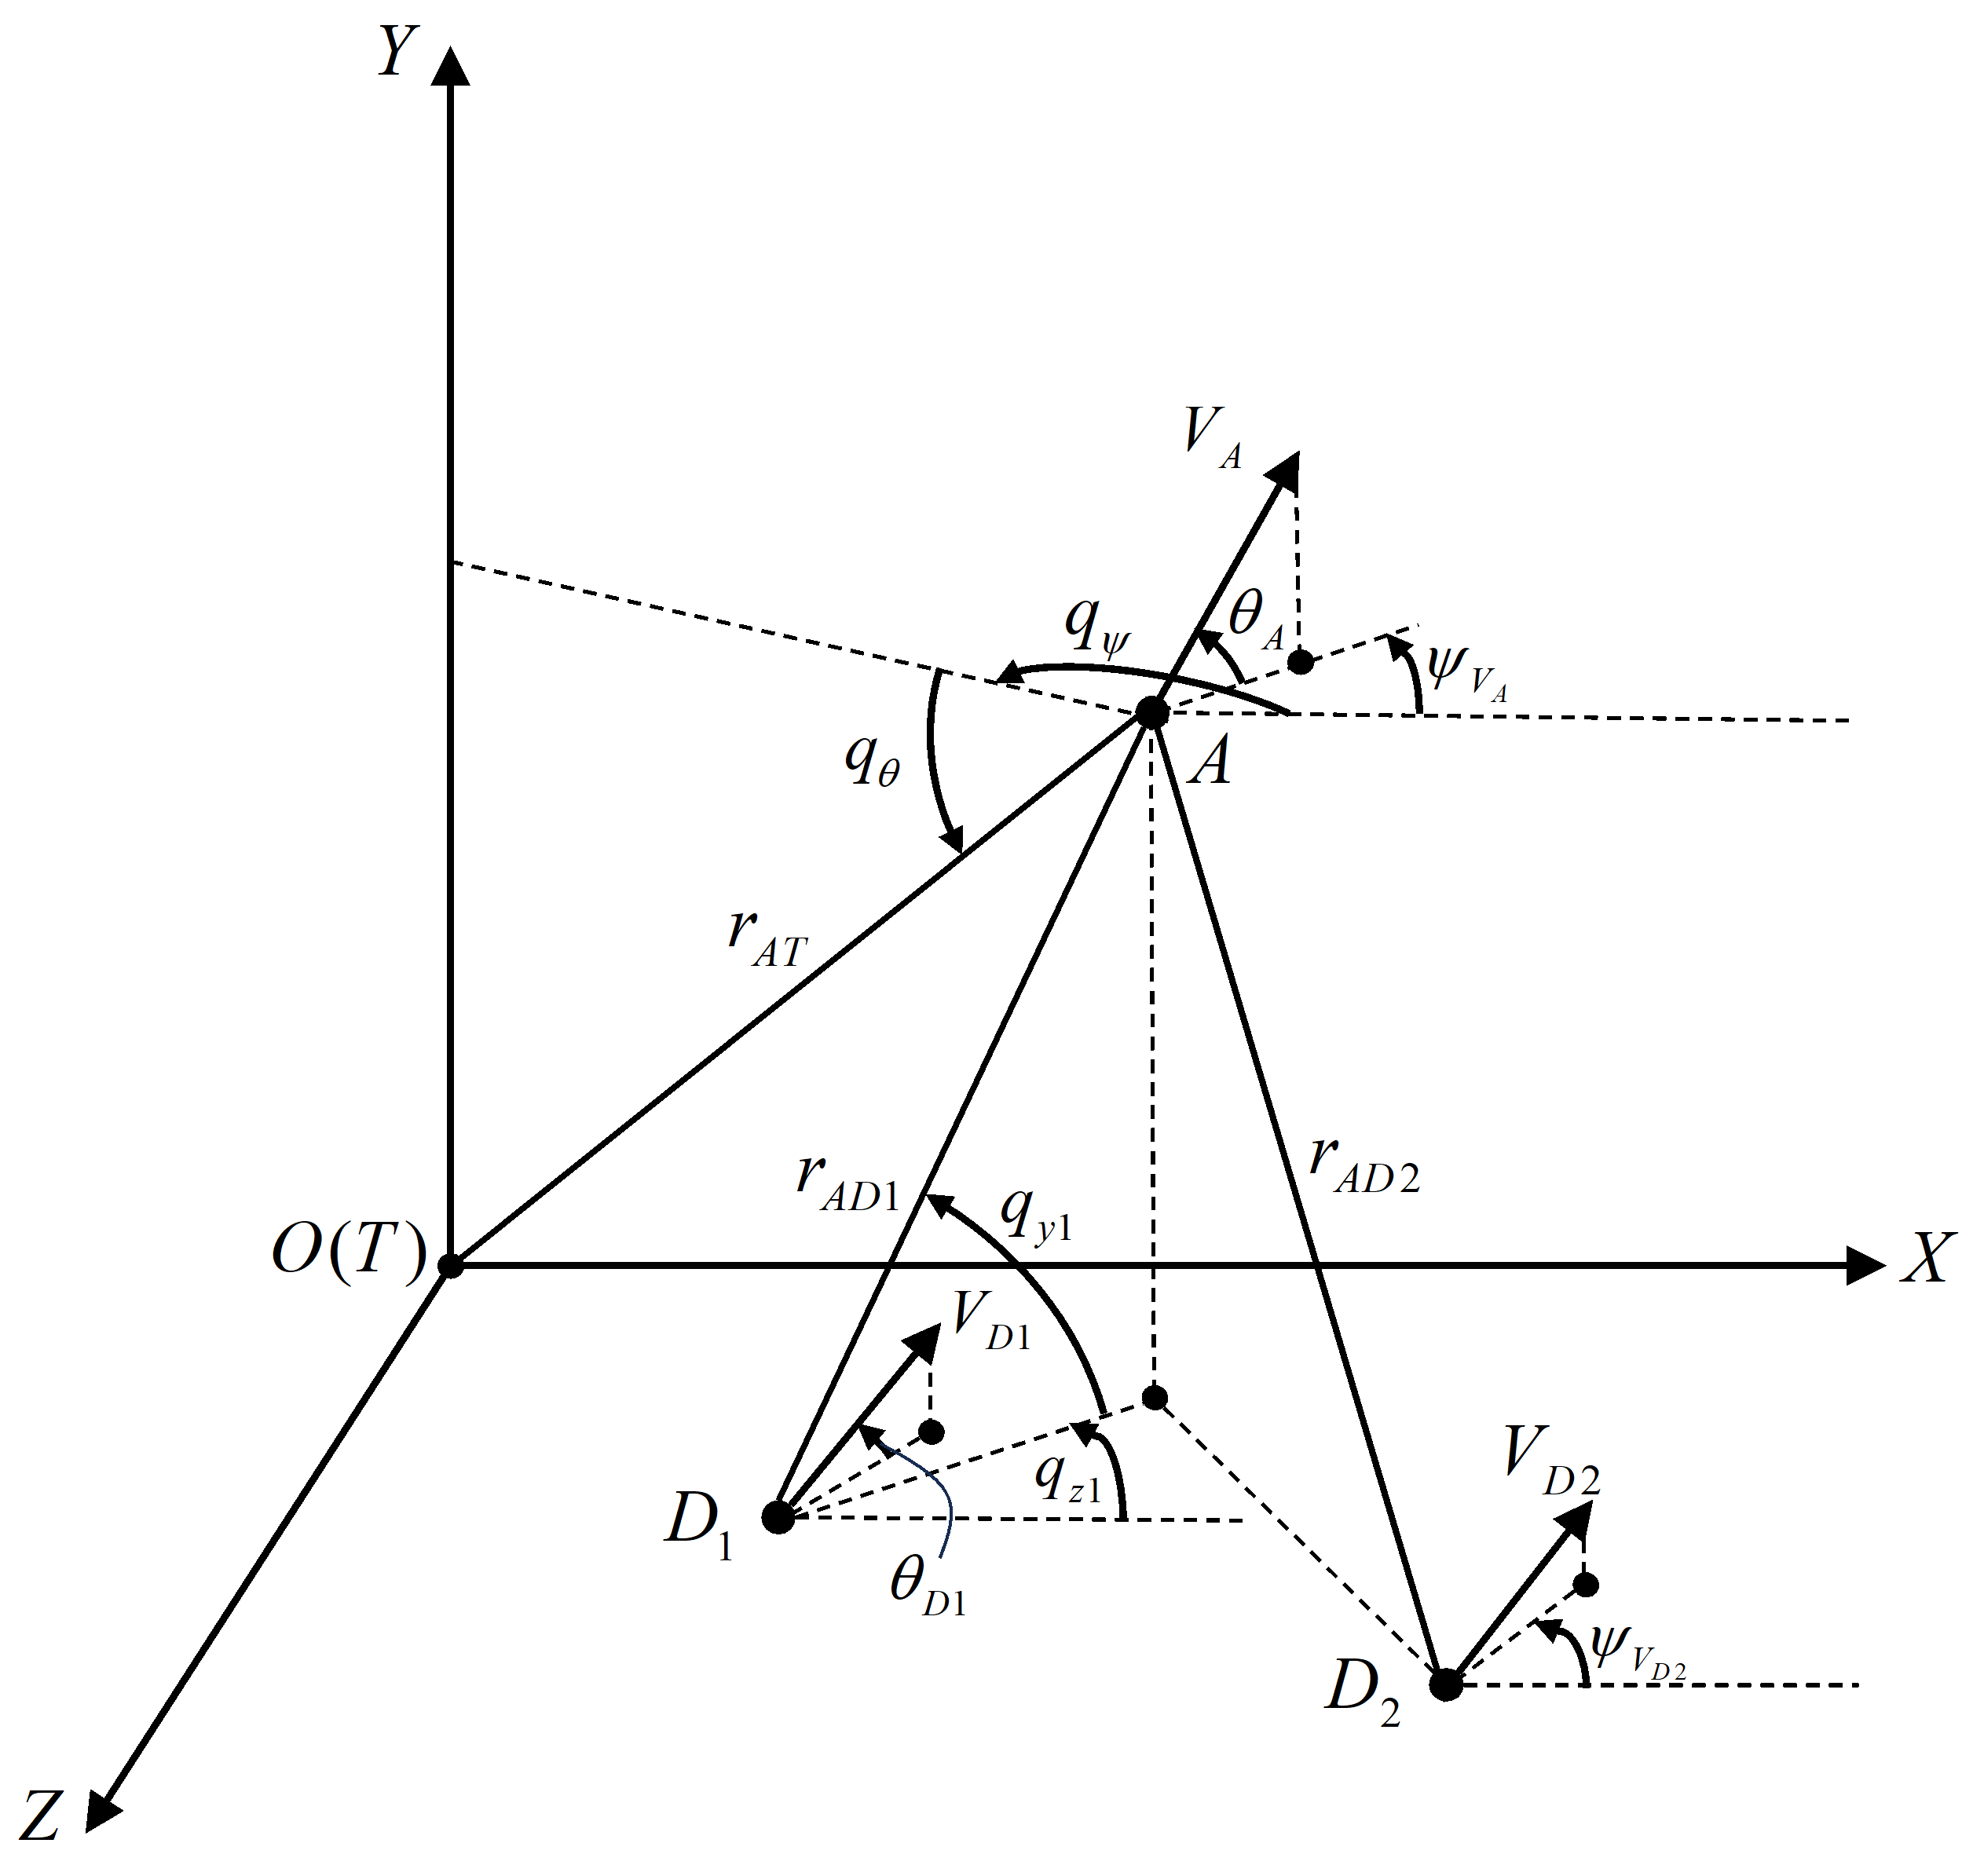
\includegraphics[width=0.92\linewidth]{fig01}
\caption{规避者-目标-非合作飞行器1-非合作飞行器2四体相对运动关系图}
\label{fig:fourbody}
\end{figure}
图~\ref{fig:fourbody}中相对位置和运动关系符号如下表~\ref{tab:symbols}所示。

\begin{table}[htbp]
\centering
\caption{图~\ref{fig:fourbody}相对位置与运动关系符号表}
\label{tab:symbols}
\small
\begin{tabularx}{\linewidth}{lXX}
\toprule
符号 & 含义 & 图~\ref{fig:fourbody}中对应正负 \\
\midrule
${r_{AT}},{r_{ADi}}$ & 规避者与目标、第i个非合作飞行器之间的距离 & 正，正 \\
${q_{yi}},{q_{zi}}$ & 第i个非合作飞行器的俯仰、偏航方向视线角 & 正，正 \\
${q_\theta },{q_\psi }$ & 规避者与目标的俯仰、偏航方向视线角 & 负，正 \\
${V_{Di}},{\theta _{Di}},{\psi _{{V_{Di}}}}$ & 第i个非合作飞行器的速度、航迹倾角和航迹偏角 & 正，正 \\
${V_A},{\theta _A},{\psi _{{V_A}}}$ & 规避者的速度、航迹倾角和航迹偏角 & 正，正 \\
${u_{ri}},{v_{ri}}$ & 规避者加速度、第i枚非合作飞行器加速度在视线坐标系x轴（正方向由第i枚非合作飞行器指向规避者）投影 & 正，正 \\
\bottomrule
\end{tabularx}
\end{table}
非合作飞行器${D_1}$, ${D_2}$与规避者$A$的相对运动方程

\begin{equation}
\label{eq:1}
\left\{ {\begin{array}{*{20}{l}}
  \begin{aligned}
& {{\dot r}_{ADi}} =  - {V_{Di}}\left[ {\cos {\theta _{Di}}\cos {q_{yi}}\cos \left( {{q_{zi}} - {\psi _{{V_{Di}}}}} \right) + \sin {\theta _{Di}}\sin {q_{yi}}} \right] +  \\
& {\text{   }}{V_A}\left[ {\cos {\theta _A}\cos {q_{yi}}\cos \left( {{q_{zi}} - {\psi _{{V_A}}}} \right) + \sin {\theta _A}\sin {q_{yi}}} \right]
\end{aligned} \\
  \begin{aligned}
& {{\dot q}_{yi}}{r_{ADi}} = {V_{Di}}\left[ {\cos {\theta _{Di}}\sin {q_{yi}}\cos \left( {{q_{zi}} - {\psi _{{V_{Di}}}}} \right) - \sin {\theta _{Di}}\cos {q_{yi}}} \right] -  \\
& {V_A}\left[ {\cos {\theta _A}\sin {q_{yi}}\cos \left( {{q_{zi}} - {\psi _{{V_A}}}} \right) - \sin {\theta _A}\cos {q_{zi}}} \right]
\end{aligned} \\
  \begin{aligned}
& {{\dot q}_{zi}}{r_{ADi}}\cos {q_{yi}} = {V_{Di}}\cos {\theta _{Di}}\sin \left( {{q_{yi}} - {\psi _{{V_{Di}}}}} \right) -  \\
& {\text{           }}{V_A}\cos {\theta _A}\sin \left( {{q_{zi}} - {\psi _{{V_A}}}} \right)
\end{aligned}
\end{array}} \right.
\end{equation}
规避者和目标相对运动方程

\begin{equation}
\label{eq:2}
\left\{ {\begin{array}{*{20}{l}}
  {{{\dot r}_{AT}} = {V_A}\left[ {\sin {q_\theta }\sin {\theta _A} - \cos \left( {{q_\psi } - {\psi _{{V_A}}}} \right)\cos {q_\theta }\cos {\theta _A}} \right]} \\ 
  {{{\dot q}_\theta } = \frac{{{V_A}\left[ {\cos {\theta _A}\sin {q_\theta }\cos \left( {{q_\psi } - {\psi _{{V_A}}}} \right) - \sin {\theta _A}\cos {q_\theta }} \right]}}{{{r_{AT}}}}} \\ 
  {{{\dot q}_\psi } = \frac{{{V_A}\cos {\theta _A}\cos \left( {{q_\psi } - {\psi _{{V_A}}}} \right)}}{{{r_{AT}}\cos {q_\theta }}}} 
\end{array}} \right.
\end{equation}
由运动学关系可得非合作飞行器与规避者视线方向相对加速度

\begin{equation}
\label{eq:3}
{\ddot r_{ADi}} = {r_{ADi}}\dot q_{yi}^2 + {r_{ADi}}\dot q_{zi}^2{\cos ^2}{q_{yi}} + {u_{ri}} - {v_{ri}}
\end{equation}
式中，${u_{ri}},{v_{ri}}$分别为规避者和第i个非合作飞行器的加速度在非合作飞行器与规避者视线坐标系（设为视线坐标系${S_i}$）x轴投影，坐标系x轴正向定义为非合作飞行器指向规避者。

目标与规避者视线方向相对加速度

\begin{equation}
\label{eq:4}
{\ddot r_{AT}} = {r_{AT}}\dot q_\theta ^2 + {r_{AT}}\dot q_\psi ^2{\cos ^2}{q_\theta } + {u_{rT}}
\end{equation}
式中，${u_{rT}}$为规避者加速度在目标与规避者视线坐标系（设为视线坐标系${S_T}$）x轴投影，坐标系x轴正向定义为目标指向规避者。

对每个飞行器，三维运动学方程为:

\begin{equation}
\label{eq:5}
\left\{ {\begin{array}{*{20}{l}}
  {{{\dot x}_j} = {V_j}\cos {\theta _j}\cos {\psi _{{V_j}}}} \\ 
  {{{\dot y}_j} = {V_j}\sin {\theta _j}} \\ 
  {{{\dot z}_j} =  - {V_j}\cos {\theta _j}\sin {\psi _{{V_j}}}} \\ 
  {{{\dot \theta }_j} = \frac{{{a_{yj}}}}{{{V_j}}}} \\ 
  {{{\dot \psi }_j} =  - \frac{{{a_{zj}}}}{{{V_j}\cos {\theta _j}}}} 
\end{array},j = A,{D_1}.{D_2}} \right.
\end{equation}
式中，$({x_i},{y_i},{z_i})$为飞行器在地面坐标系位置坐标；${a_{yj}}$, ${a_{zj}}$分别表示垂直于飞行器速度矢量的铅垂方向和水平方向的法向加速度。

由视线方向相对加速度关系式可知，规避者与第i枚非合作飞行器的加速度在视线坐标系${S_i}$的x轴投影${u_{ri}}$和${v_{ri}}$，与各自法向加速度${a_{yA}}$,${a_{zA}}$和${a_{yDi}}$,${a_{zDi}}$存在坐标转换关系。设地面坐标系到视线坐标系${S_i}$的转换矩阵为${\mathbf{L}}({q_{yi}},{q_{zi}})$，地面坐标系到航迹坐标系的转换矩阵为${\mathbf{L}}(\theta ,{\psi _V})$，则两者的投影关系可表示为

\begin{equation}
\label{eq:6}
{u_{ri}} = \left[ {\begin{array}{*{20}{c}}
  1&0&0 
\end{array}} \right]{\mathbf{L}}({q_{yi}},{q_{zi}}){{\mathbf{L}}^{ - 1}}({\theta _A},{\psi _{{V_A}}})\left[ {\begin{array}{*{20}{c}}
  0 \\ 
  {{a_{yA}}} \\ 
  {{a_{zA}}} 
\end{array}} \right]
\end{equation}
\begin{equation}
\label{eq:7}
{v_{ri}} = \left[ {\begin{array}{*{20}{c}}
  1&0&0 
\end{array}} \right]{\mathbf{L}}({q_{yi}},{q_{zi}}){{\mathbf{L}}^{ - 1}}({\theta _{Di}},{\psi _{{V_{Di}}}})\left[ {\begin{array}{*{20}{c}}
  0 \\ 
  {{a_{yDi}}} \\ 
  {{a_{zDi}}} 
\end{array}} \right]
\end{equation}
其中转换矩阵的具体形式与三维空间坐标系转换的通用定义一致，此处不再赘述。同理，设地面坐标系到视线坐标系${S_T}$的转换矩阵为${\mathbf{L}}({q_\theta },{q_\psi })$，则规避者与目标的加速度在坐标系${S_T}$的x轴投影

\begin{equation}
\label{eq:8}
{u_{rT}} = \left[ {\begin{array}{*{20}{c}}
  1&0&0 
\end{array}} \right]{\mathbf{L}}({q_\theta },{q_\psi }){{\mathbf{L}}^{ - 1}}({\theta _A},{\psi _{{V_A}}})\left[ {\begin{array}{*{20}{c}}
  0 \\ 
  {{a_{yA}}} \\ 
  {{a_{zA}}} 
\end{array}} \right]
\end{equation}
\begin{assumption}
非合作飞行器均采用经典比例导引（PN）制导律，其加速度指令为：
\end{assumption}
\begin{equation}
\label{eq:9}
\left[ {\begin{array}{*{20}{c}}
  {{a_{yDi}}} \\ 
  {{a_{zDi}}} 
\end{array}} \right] = \left[ {\begin{array}{*{20}{c}}
  {{K_{Di}}{V_{Di}}{{\dot q}_{yi}}} \\ 
  { - {K_{Di}}{V_{Di}}{{\dot q}_{zi}}\cos {\theta _{Di}}} 
\end{array}} \right]
\end{equation}
式中，${K_{Di}}$为第i枚非合作飞行器比例导引系数。

\begin{assumption}
两个非合作飞行器性能指标相同，即${K_{{D_1}}} = {K_{{D_2}}} = {K_D}$, ${V_{{D_1}}} = {V_{{D_2}}} = {V_D}$，以及期望规避距离满足$d_1^* = d_2^* = {d^*}$.
\end{assumption}
\subsection{线性化状态空间模型}
将式\eqref{eq:6}、\eqref{eq:7}及其中的转换矩阵代入式\eqref{eq:3}得

\begin{equation}
\label{eq:10}
\begin{gathered}
  {{\ddot r}_{ADi}} = {r_{ADi}}\left( {\dot q_{yi}^2 + \dot q_{zi}^2{{\cos }^2}{q_{yi}}} \right) - \cos {q_{yi}}\sin \left( {{q_{zi}} - {\psi _{{V_A}}}} \right){a_{zA}} +  \\ 
  {a_{yA}}\left[ { - \cos {q_{yi}}\sin {\theta _A}\cos \left( {{q_{zi}} - {\psi _{{V_A}}}} \right) + \sin {q_{yi}}\cos {\theta _A}} \right] -  \\ 
  {a_{yDi}}\left[ { - \cos {q_{yi}}\sin {\theta _{Di}}\cos \left( {{q_{zi}} - {\psi _{{V_{Di}}}}} \right) + \sin {q_{yi}}\cos {\theta _{Di}}} \right] +  \\ 
  \cos {q_{yi}}\sin \left( {{q_{zi}} - {\psi _{{V_{Di}}}}} \right){a_{zDi}} \\ 
\end{gathered}
\end{equation}
同理，将式\eqref{eq:8}及其中的转换矩阵代入式\eqref{eq:4}得

\begin{equation}
\label{eq:11}
\begin{gathered}
  {{\ddot r}_{AT}} = {r_{AT}}\left( {\dot q_\theta ^2 + \dot q_\psi ^2{{\cos }^2}{q_\theta }} \right) + (\cos {q_\theta }\cos {q_\psi }\sin {\theta _A} + \sin {q_\theta }\cos {\theta _A}){a_{yA}} +  \\ 
  {a_{zA}}(\sin {\theta _A}\sin {\psi _{{V_A}}}\sin {q_\theta } - \cos {\theta _A}\sin {\psi _{{V_A}}}\cos {q_\theta }\cos {q_\psi } - \cos {\psi _{{V_A}}}\cos {q_\theta }\sin {q_\psi }) \\ 
\end{gathered}
\end{equation}
定义状态变量${x_i} = {\left[ {\begin{array}{*{20}{c}}
  {{r_{ADi}}}&{{{\dot r}_{ADi}}} 
\end{array}} \right]^T}$，控制变量\[{u_A} = {\left[ {\begin{array}{*{20}{c}}
  {{a_{yA}}}&{{a_{zA}}} 
\end{array}} \right]^T}\]，则可得规避者与第i个非合作飞行器交互的状态空间方程

\begin{equation}
\label{eq:12}
\mathop {{x_i}}\limits^. (t) = {{\mathbf{A}}_i}{x_i}(t) + {{\mathbf{B}}_i}{u_A}(t) + {{\mathbf{C}}_i} + {v_i}
\end{equation}
式中，\[{{\mathbf{A}}_i} = \left[ {\begin{array}{*{20}{c}}
  0&1 \\ 
  {\dot q_{yi}^2 + \dot q_{zi}^2{{\cos }^2}{q_{yi}}}&0 
\end{array}} \right]\],${{\mathbf{B}}_i} = \left[ {\begin{array}{*{20}{c}}
  0&0 \\ 
  {{B_{1i}}}&{{B_{2i}}} 
\end{array}} \right]$,${{\mathbf{C}}_i} = \left[ {\begin{array}{*{20}{c}}
  0 \\ 
  {{C_{1i}}} 
\end{array}} \right]$，其中

\begin{equation}
\label{eq:13}
\left\{ {\begin{array}{*{20}{l}}
  {{B_{1i}} = \sin {q_{yi}}\cos {\theta _A} - \cos {q_{yi}}\sin {\theta _A}\cos \left( {{q_{zi}} - {\psi _{{V_A}}}} \right)} \\ 
  {{B_{2i}} = \cos {q_{yi}}\sin \left( {{q_{zi}} - {\psi _{{V_A}}}} \right)} \\ 
  {{C_{1i}} = \cos {q_{yi}}\sin \left( {{q_{zi}} - {\psi _{{V_{Di}}}}} \right){a_{zDi}} + [\cos {q_{yi}}\sin {\theta _{Di}}\cos \left( {{q_{zi}} - {\psi _{{V_{Di}}}}} \right) - \sin {q_{yi}}\cos {\theta _{Di}}]{a_{yDi}}} 
\end{array}} \right.
\end{equation}
定义状态变量${x_{AT}} = {\left[ {\begin{array}{*{20}{c}}
  {{r_{AT}}}&{{{\dot r}_{AT}}} 
\end{array}} \right]^T}$，则可得规避者与目标的相对状态空间方程

\begin{equation}
\label{eq:14}
{\dot x_{AT}}(t) = {{\mathbf{A}}_T}{x_{AT}}(t) + {{\mathbf{B}}_T}{u_A}(t)
\end{equation}
式中，\[{{\mathbf{A}}_T} = \left[ {\begin{array}{*{20}{c}}
  0&1 \\ 
  {\dot q_\theta ^2 + \dot q_\psi ^2{{\cos }^2}{q_\theta }}&0 
\end{array}} \right]\],${{\mathbf{B}}_T} = \left[ {\begin{array}{*{20}{c}}
  0&0 \\ 
  {{B_{1T}}}&{{B_{2T}}} 
\end{array}} \right]$，其中

\begin{equation}
\label{eq:15}
\left\{
\begin{aligned}
& {B_{1T}} = \cos {q_\theta }\cos {q_\psi }\sin {\theta _A} + \sin {q_\theta }\cos {\theta _A} \\
& {B_{2T}} = \sin {\theta _A}\sin {\psi _{{V_A}}}\sin {q_\theta } - \cos {\theta _A}\sin {\psi _{{V_A}}}\cos {q_\theta }\cos {q_\psi } - \cos {\psi _{{V_A}}}\cos {q_\theta }\sin {q_\psi }
\end{aligned}
\right.
\end{equation}
\begin{remark}
系统\eqref{eq:12}-\eqref{eq:15}是线性时变的(LTV)，但在每个离散制导周期内，矩阵${{\mathbf{A}}_i}$, ${{\mathbf{B}}_i}$, ${{\mathbf{C}}_i}$, ${{\mathbf{A}}_T}$, ${{\mathbf{B}}_T}$可近似视为时不变。该拟冻结系数假设在工程实践中已得到广泛验证，并为第3节的在线参数辨识提供了数学基础。
\end{remark}
辨识目标汇总. 待辨识的非平凡元素如表~\ref{tab:nontrivial}所示：

\begin{table}[htbp]
\centering
\caption{待辨识非平凡元素}
\label{tab:nontrivial}
\small
\begin{tabularx}{\linewidth}{lXXX}
\toprule
方程 & 矩阵 & 元素 & 物理含义 \\
\midrule
式\eqref{eq:12} & ${{\mathbf{A}}_i}$ & $A_{21}^{(i)} = \dot q_{yi}^2 + \dot q_{zi}^2{\cos ^2}{q_{yi}}$ & 视线角速率耦合 \\
式\eqref{eq:12} & ${B_i}$ & ${B_{1i}},{B_{2i}}$ & 规避者加速度投影系数（非合作飞行器方向） \\
式\eqref{eq:12} & ${C_i}$ & ${C_i}$ & 非合作飞行器机动加速度偏置 \\
式\eqref{eq:15} & ${{\mathbf{A}}_T}$ & $A_{21}^{(T)} = \dot q_\theta ^2 + \dot q_\psi ^2{\cos ^2}{q_\theta }$ & 目标-规避者视线角速率耦合 \\
式\eqref{eq:15} & ${B_T}$ & ${B_{1T}},{B_{2T}}$ & 规避者加速度投影系数（目标方向） \\
\bottomrule
\end{tabularx}
\end{table}
\begin{remark}
a（测量噪声）. 在实际应用中，式\eqref{eq:13}和\eqref{eq:15}中的矩阵元素由机载传感器/IMU测量得到，而非由无噪声理想运动学计算。测量得到的视线角、视线角速率与飞行器航迹倾角/航向角均叠加零均值高斯白噪声：
\end{remark}
\begin{equation}
\label{eq:16}
\begin{gathered}
  {{\tilde q}_\alpha } = {q_\alpha } + {\nu _{q,\alpha }},\quad {\nu _{q,\alpha }}\sim \mathcal{N}(0,\sigma _q^2), \hfill \\
  {{\tilde \dot q}_\alpha } = {{\dot q}_\alpha } + {\nu _{\dot q,\alpha }},\quad {\nu _{\dot q,\alpha }}\sim \mathcal{N}(0,\sigma _{\dot q}^2), \hfill \\
  {{\tilde \theta }_j} = {\theta _j} + {\nu _{\theta ,j}},\quad {\nu _{\theta ,j}}\sim \mathcal{N}(0,\sigma _\theta ^2), \hfill \\
  {{\tilde \psi }_{{V_j}}} = {\psi _{{V_j}}} + {\nu _{\psi ,j}},\quad {\nu _{\psi ,j}}\sim \mathcal{N}(0,\sigma _\psi ^2), \hfill \\ 
\end{gathered}
\end{equation}
式中，$\alpha  \in \left\{ {{y_i},{z_i},\theta ,\psi } \right\}$分别对应与NCV（非合作飞行器）视线和与目标视线各通道，$j \in \left\{ {A,{D_1},{D_2}} \right\}$. 该传感器噪声模型即为第3节在线参数辨识框架的出发点，该框架从相对距离动力学中恢复矩阵元素，而不依赖对噪声敏感的解析式\eqref{eq:13}/\eqref{eq:15}。

\subsection{最优问题建立}
为降低系统阶次并简化求解，引入ZEM $z(t)$。定义规避者与第i个非合作飞行器的ZEM

\begin{equation}
\label{eq:17}
{z_i}(t) = \left[ {\begin{array}{*{20}{c}}
  1&0 
\end{array}} \right]\Omega \left( {{t_{fi}},t} \right){x_i}(t)
\end{equation}
式中，状态转移矩阵

\begin{equation}
\label{eq:18}
\Omega \left( {{t_{fi}},t} \right) = {e^{{A_i}\left( {{t_{fi}} - t} \right)}} = \left[ {\begin{array}{*{20}{c}}
  {\cosh ({{\dot Q}_i}{t_{{\text{go,i}}}})}&{\frac{{\sinh ({{\dot Q}_i}{t_{{\text{go,i}}}})}}{{{{\dot Q}_i}}}} \\ 
  {{{\dot Q}_i}\sinh ({{\dot Q}_i}{t_{{\text{go,i}}}})}&{\cosh ({{\dot Q}_i}{t_{{\text{go,i}}}})} 
\end{array}} \right]
\end{equation}
其中，${\dot Q_i} = \sqrt {\dot q_{yi}^2 + \dot q_{zi}^2{{\cos }^2}{q_{yi}}} $为视线角速度合成量，${t_{go,i}} = {t_{fi}} - t$为剩余飞行时间。利用状态转移矩阵性质$\dot \Omega \left( {{t_{fi}},t} \right) =  - \Omega \left( {{t_{fi}},t} \right){A_i}$，对式\eqref{eq:17}求导整理可得

\begin{equation}
\label{eq:19}
{\dot z_i}(t) = {\varphi _i}(t)b_i^T{u_A}(t) - {\varphi _i}(t){v_{ri}}
\end{equation}
式中，

\begin{equation}
\label{eq:20}
\left\{
\begin{aligned}
& {\varphi _i}(t) = \frac{{{e^{{{\dot Q}_i}{t_{go,i}}}} - {e^{ - {{\dot Q}_i}{t_{go,i}}}}}}{{2{{\dot Q}_i}}} \\
& {b_i} = {\left[ {\begin{array}{*{20}{c}}
  {{B_{1i}}}&{{B_{2i}}}
\end{array}} \right]^T}
\end{aligned}
\right.
\end{equation}
同理可得规避者与目标的ZEM导数

\begin{equation}
\label{eq:21}
{\dot z_T}(t) = {\varphi _T}(t)b_t^T{u_A}(t)
\end{equation}
式中，

\begin{equation}
\label{eq:22}
\left\{
\begin{aligned}
& {\varphi _T}(t) = \frac{{{e^{{{\dot Q}_T}{t_{go,T}}}} - {e^{ - {{\dot Q}_T}{t_{go,T}}}}}}{{2{{\dot Q}_T}}} \\
& {b_t} = {\left[ {\begin{array}{*{20}{c}}
  {{B_{1T}}}&{{B_{2T}}}
\end{array}} \right]^T}
\end{aligned}
\right.
\end{equation}
其中，${\dot Q_T} = \sqrt {\dot q_\theta ^2 + \dot q_\psi ^2{{\cos }^2}{q_\theta }} $,${t_{go,T}} = {t_{fT}} - t$.

本文智能规避算法的核心目标是在保证成功规避两枚非合作飞行器的同时，最小化机动能量消耗，并避免过度机动影响后续目标到达。为此，构建如下二次型性能指标函数

\begin{equation}
\label{eq:23}
\mathop {\min }\limits_{{u_A}} J = \sum\nolimits_{i = 1}^2 {\frac{{{w_i}}}{2}{{\left[ {z\left( {{t_{fi}}} \right) - d_i^*} \right]}^2}}  + \frac{{{w_E}}}{2}\int_{{t_0}}^{{t_f}} {u_A^T{u_A}d\tau {\text{ + }}\frac{{{w_T}}}{2}z_T^2\left( {{t_{fT}}} \right)}
\end{equation}
式中，${w_i} > 0$为规避ZEM权重，${w_E} > 0$为控制能量权重，${w_T} > 0$为目标到达ZEM权重，$d_i^*$为规避者与第i个非合作飞行器的期望规避距离，通常设定为略大于非合作飞行器作用半径。${t_f} = \max ({t_{f1}},{t_{f2}})$为全局规避终止时刻。为体现对两枚非合作飞行器的均衡规避需求，设${w_1} + {w_2} = w$（$w$为一正常数），且${w_1}$, ${w_2}$满足

\begin{equation}
\label{eq:24}
\left\{
\begin{aligned}
& {w_1} = w \cdot \frac{1}{{1 + {e^{ - \gamma }}}} \\
& {w_2} = w - {w_1} = w \cdot \frac{{{e^{ - \gamma }}}}{{1 + {e^{ - \gamma }}}}
\end{aligned}
\right.
\end{equation}
\begin{problem}[一体化最优规避与制导]
给定状态空间方程\eqref{eq:12}与\eqref{eq:14}，在运动学\eqref{eq:1}–\eqref{eq:5}约束下，求使性能指标\eqref{eq:23}最小的最优控制$u_A^*(t)$。
\end{problem}
